\documentclass[12pt]{article}
\usepackage[parfill]{parskip}
\usepackage{amsmath}
\usepackage{amssymb}
\usepackage{bm}
\usepackage{enumerate}
\usepackage{fancyvrb}
\usepackage[top=1in, bottom=1in, left=1in, right=1in]{geometry}
\usepackage{hyperref}
\hypersetup{
    colorlinks=true,
}
\usepackage{placeins}
\usepackage{tikz}
\usepackage{tikzsymbols}
\usepackage{todonotes}
\usepackage{bbm}
\usepackage{color}
\usepackage{enumitem}
\usepackage{xcolor}
\newcommand{\rmn}[1]{{\textcolor{blue}{\bf [{\sc rmn:} #1]}}}
\DeclareMathOperator*{\argmax}{arg\,max}
\usepackage{algorithmicx}
\usepackage{algorithm}
\usepackage{algpseudocode}
\usepackage{multirow}
\usepackage{rotating}

\usetikzlibrary{positioning,calc}
%%%%%%%%%
\usepackage[most]{tcolorbox}
\newtcolorbox[]{solution}[1][]{%
    breakable,
    enhanced,
    colback=white,
    title=Solution,
    #1
}
%%%%%%%%%%
\title{10-703 Deep Reinforcement Learning and Control\\
  Assignment 3\\
  Fall 2018 \\  
}
\author{ielshar \\ mharding}
\date{October 26, 2018}
\begin{document}

\maketitle

\section*{Problem 1: Reinforce}
\begin{enumerate}
	\item  Describe your implementation:
	\begin{itemize}
		\item Neural Network Architecture:  same as given in JSON file.
		\item Learning rate: 0.001
		\item Discount factor $\gamma: 1$
	\end{itemize}
	\item 
		\begin{figure}[H]
		\begin{center} 
			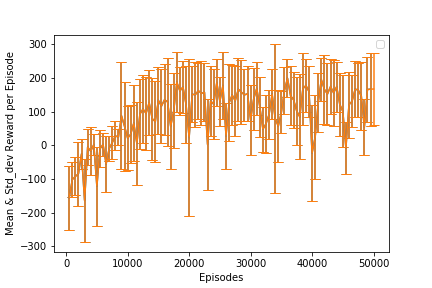
\includegraphics[scale=.73]{figures/Reinforce_LC_50.png}
		\end{center}
		\caption{Reinforce Algorithm: learning curve - Every k=500 episodes the current policy is tested on 100 episodes. The plot shows the mean and standard deviation of each of this tests.  } 	\label{1}%
	\end{figure}
\end{enumerate}

Figure \ref{1} above shows that our agent was able to achieve a mean reward of 200  or slightly more or less at several points (after 19000, 36000, 41500 episodes) through out the training. Since no baseline was used in our Reinforce algorithm one can see that the test results have a high variance. This is somehow expected though as the total return at the end of episode varies highly from one episode to another.

\section*{Problem 2: Advantage-Actor Critic}
\begin{enumerate}
\item Implementation details:
% Table generated by Excel2LaTeX from sheet 'Sheet2'
\begin{table}[H]
  \centering
  \caption{A2C Implementation}
    \begin{tabular}{|c|p{11.085em}|l|}
    \hline
    \multicolumn{3}{|c|}{A2C } \\
    \hline
    N     & Settings & \multicolumn{1}{p{16em}|}{value} \\
    \hline
    \multirow{4}[8]{*}{1} & Actor NN Architecture  & \multicolumn{1}{p{16em}|}{Same as given in JSON file} \\
\cline{2-3}          & Critiic NN Architecture  & \multicolumn{1}{p{16em}|}{MLP with 3 layers each with 20 hidden units and relu activation} \\
\cline{2-3}          & Actor learning rate & 0.001 \\
\cline{2-3}          & Critic learning rate & 0.001 \\
    \hline
    \multirow{4}[8]{*}{20} & Actor NN Architecture  & \multicolumn{1}{p{16em}|}{Same as given in JSON file} \\
\cline{2-3}          & Critiic NN Architecture  & \multicolumn{1}{p{16em}|}{MLP with 3 layers each with 20 hidden units and relu activation} \\
\cline{2-3}          & Actor learning rate & 0.001 \\
\cline{2-3}          & Critic learning rate & 0.001 \\
    \hline
    \multirow{4}[8]{*}{50} & Actor NN Architecture  & \multicolumn{1}{p{16em}|}{Same as given in JSON file} \\
\cline{2-3}          & Critiic NN Architecture  & \multicolumn{1}{p{16em}|}{MLP with 3 layers each with 20 hidden units and relu activation} \\
\cline{2-3}          & Actor learning rate & 0.001 \\
\cline{2-3}          & Critic learning rate & 0.001 \\
    \hline
    \multirow{4}[7]{*}{100} & Actor NN Architecture  & \multicolumn{1}{p{16em}|}{Same as given in JSON file} \\
\cline{2-3}          & Critiic NN Architecture  & \multicolumn{1}{p{16em}|}{MLP with 3 layers each with 20 hidden units and relu activation} \\
\cline{2-3}          & Actor learning rate & 0.001 \\
\cline{2-3}          & Critic learning rate & 0.001 \\
\hline
    \end{tabular}%
  \label{2}%
\end{table}%
\item  Plots:
\begin{itemize}
	\item  N=20
		\begin{figure}[H]
			\begin{center} 
				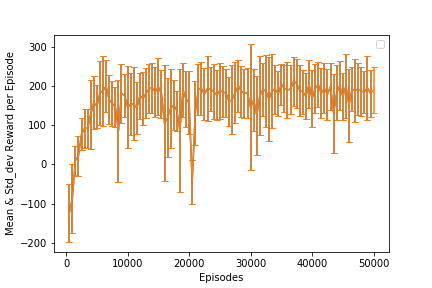
\includegraphics[scale=.73]{figures/A2C_LC_N=20_50.png}
			\end{center}
			\caption{A2C Algorithm N=20: learning curve - Every k=500 episodes the current policy is tested on 100 episodes. The plot shows the mean and standard deviation of each of this tests.  } 	\label{4}%
		\end{figure}
	\item N=50
		\begin{figure}[H]
			\begin{center} 
				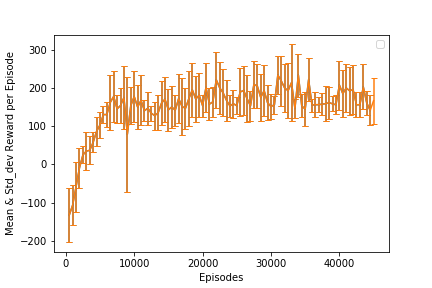
\includegraphics[scale=.73]{figures/A2C_LC_N=50_45.png}
			\end{center}
			\caption{A2C Algorithm N=50: learning curve - Every k=500 episodes the current policy is tested on 100 episodes. The plot shows the mean and standard deviation of each of this tests.  } 	\label{5}%
		\end{figure}
	\item N=100
		\begin{figure}[H]
			\begin{center} 
				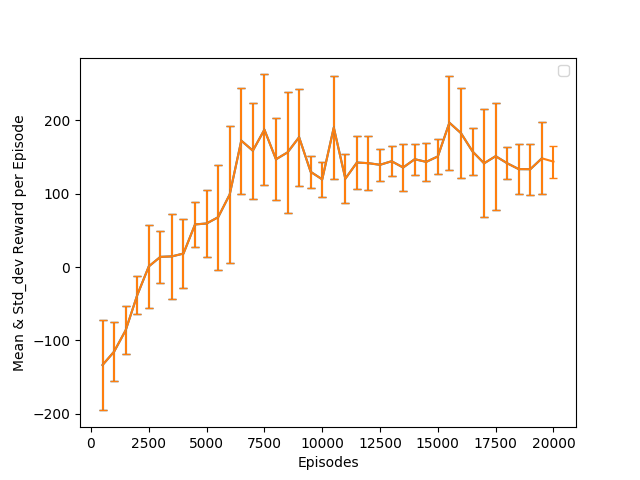
\includegraphics[scale=.73]{figures/A2C_LC_N=100_20.png}
			\end{center}
			\caption{A2C Algorithm N=100: learning curve - Every k=500 episodes the current policy is tested on 100 episodes. The plot shows the mean and standard deviation of each of this tests.  } 	\label{6}%
		\end{figure}	 
	\end{itemize}

\item  Reinforce and A2C comparisons:\\
			Compared to Reinforce, n-steps A2Cs have much lower variance and accelerated learning. This is due to the critic which replaces G in reinforce. 


\end{enumerate}




\end{document}